\documentclass[11pt]{article}
\usepackage[utf8]{inputenc}
\usepackage{xcolor,comment, subfiles, graphicx, caption, longtable, subfig, fancyhdr}
\usepackage{float} %Used to force images to appear in the section in which it's declared
\usepackage[hidelinks]{hyperref}
\usepackage{parskip}
\usepackage[shortlabels]{enumitem}
\usepackage{multirow}
\usepackage{color}
\usepackage[toc,page]{appendix}
\usepackage{float}
\usepackage[a4paper,width=150mm,top=25mm,bottom=25mm]{geometry}
\usepackage{longtable}
\usepackage{colortbl}
\usepackage{xcolor}
\usepackage{color}
\usepackage{amsfonts}
\usepackage{amssymb}
\usepackage{amsmath}
\usepackage{cancel}


\newcommand{\subf}[2]{%
  {\small\begin{tabular}[t]{@{}c@{}}
   \mbox{}\\[-\ht\strutbox]
   #1\\#2
   \end{tabular}}%
}

\title{DASA - Project}
\makeatletter

\begin{document}

\setlength{\parskip}{1em}

\begin{titlepage}
\centering
\vfill
{

\includegraphics[width =\linewidth, height = 4cm, keepaspectratio]{PolitecnicoLogo.png}
\label{fig:PolitecnicoLogo}
\large \\[2ex]M.Sc. Computer Science and Engineering\\
\large Data Analysis for Smart Agriculture\\[12ex]
\huge
Data Analysis On An Eggs Farm\\[1.5ex]
\large
\vspace{10mm}

\vspace{15mm}
\normalsize

\vspace{30mm}

\begin{tabular}{lclcl}
    Davide Canali & - & 10674880 & - & davide1.canali@polimi.it\\
    Matteo Cordioli & - & 00000000 & - & matteo.cordioli@polimi.it\\
    Federico Camilletti & - & 10619856 & - & federico.camilletti@polimi.it\\
    Shakiba Shahidiani  & - & 00000000 & - & shakiba.shahidiani@polimi.it\\
\end{tabular}

\vspace{30mm}

\@date\\[2.5ex]
}
\end{titlepage}

\makeatother
\tableofcontents
\newpage

\section{Introduction}
In this study, we are going to analyze data from an eggs farm near Mantova to see if it's possible to improve both animal welfare and farmer revenue.

The farm under analysis is [//TODO INSERT NAME] and has around 40'000 chickens that produce organic eggs. We have the data starting from 2014, the production of eggs is divided into cycles lasting about 13 - 15 months each. We have 5 complete cycles and the current 2022 cycle. The first 2 cycles (called X and Y) are non-organic which means the chickens are treated differently from the last 4 cycles (Z, A, B, C) which are organic.

Upon talking with the farmer we focus our attention on 3 main topics which involve:
\begin{itemize}
    \item Understanding the mortality between different cycles and organic with non-organic.
    \item Improve the welfare of the chickens.
    \item Quantify the monetary loss when a chicken dies at the start of the cycle.
\end{itemize}

\section{Data Collection}
The farmer collected the data thanks to sensors and by inspecting the barns each day. Before cycle A the data were only collected in paper spreadsheets and had to be imported in a digital format.

\section{Data Cleaning}
Before starting to analyze the data we cleaned them.
In all the cycles we performed these next steps:
\begin{itemize}
    \item Removed tail and head (20 rows each more or less).
    \item Adjusted feed and water consumption to correct typos and switchboard errors.
    \item Adjusted eggs production when \% of laid when above 100\%, distributed in the days before assuming that those eggs were not collected.
    \item Adjusted death count to match the delta of death at the end of the cycle.
    \item Checked that the difference between the total amount of eggs produced and the number of eggs sold was less than 0.6\%.
\end{itemize}

Specifically, in cycle A we also adjust a series of missing data regarding the water consumption adding them following the cycle distribution.

//TODO Teo add what u did in cycles Y and X


\section{Analysis of Each Cycle}
\subsection{Cycle A}
\begin{center}
    \begin{tabular}{|c | c | c | c | c | c|} 
        \hline
        \textbf{Arrival date} & \textbf{\#Chickens} & \textbf{Frist Laid} & \textbf{End of cycle} & \textbf{Organic} & \textbf{\#Eggs}\\ [0.5ex] 
        \hline
        19/7/2018 & 42.009 & 1/9/2018 & 19/5/2020 & Yes & 20.208.086\\
        \hline
    \end{tabular}
\end{center}
Significant features:
\begin{itemize}
    \item Average Percentage of Laid Eggs each day: 83,8\%
    \item Average Percentage of Death each day: 0,044\%
    \item Average Temperature during the cycle: 12,99 °C
    \item Average Humidity during the cycle: 74,55\%
\end{itemize}

Cluster:
\begin{center}
\begin{tabular}{|c|c|}
    \hline
    \subf{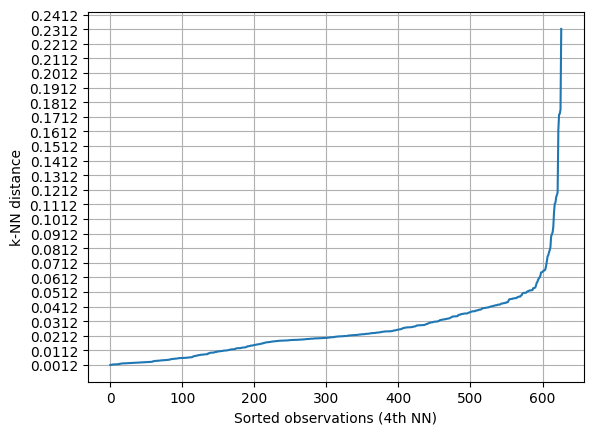
\includegraphics[width=70mm]
    {../Results/Two_clusters_division/CycleA/Density_epsilon.png}}
         {k-NN distance to find $\epsilon$}
    &
    \subf{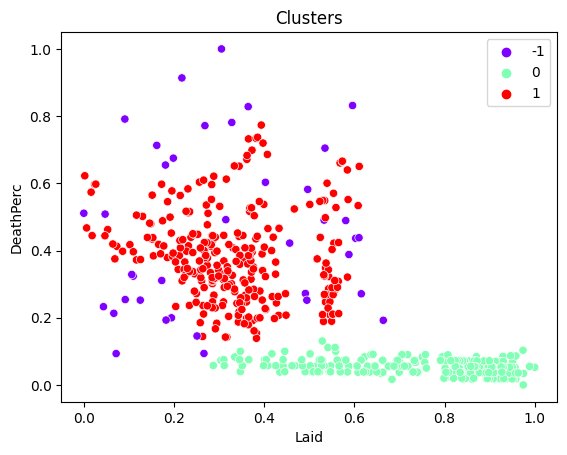
\includegraphics[width=70mm]
    {../Results/Two_clusters_division/CycleA/Density_scatter_merged.png}}
         {Density scatter plot merged}
    \\
    \hline
    \subf{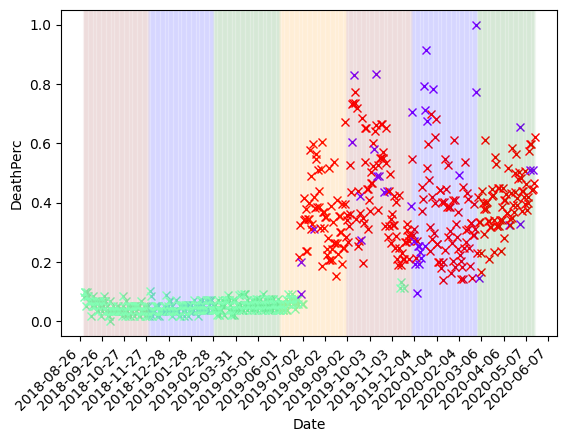
\includegraphics[width=70mm]
    {../Results/Two_clusters_division/CycleA/Density_plot_death.png}}
         {Percentage of death}
    &
    \subf{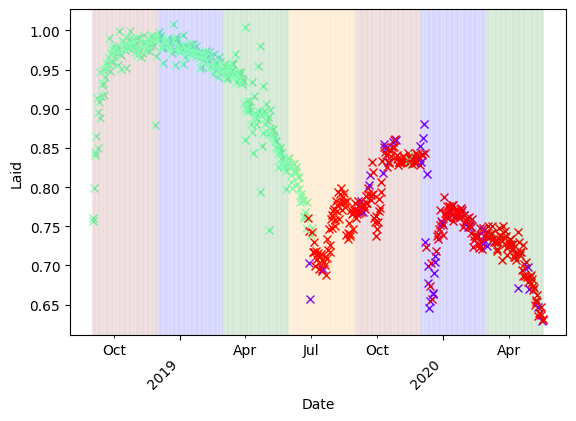
\includegraphics[width=70mm]
    {../Results/Two_clusters_division/CycleA/Density_plot_laied.png}}
         {Percentage of laid eggs}
    \\
    \hline
\end{tabular}
\end{center}

\subsection{Cycle B}
\begin{center}
    \begin{tabular}{| c | c | c | c | c | c | c |} 
        \hline
        Arrival date & \#Chickens & Frist Laid & End of cycle & Organic & \#Eggs\\ [0.5ex] 
        \hline
        09/08/2020 & 42.098 & 24/09/2020 & 02/05/2022 & Yes & 18.392.640\\ 
        \hline
    \end{tabular}
\end{center}

Significant features:
\begin{itemize}
    \item Average Percentage of Laid Eggs each day: 81,39\%
    \item Average Percentage of Death each day: 0,0494\%
    \item Average Temperature during the cycle: 11,81 °C
    \item Average Humidity during the cycle: 73,24\%
\end{itemize}

Cluster:
\begin{center}
\begin{tabular}{|c|c|}
    \hline
    \subf{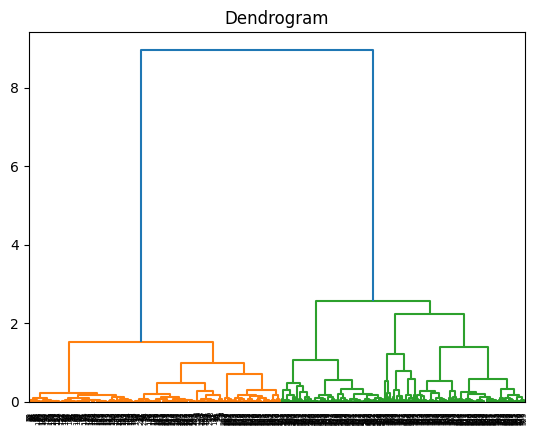
\includegraphics[width=70mm]
    {../Results/Two_clusters_division/CycleB/Hierarchical_dendogram.png}}
         {Dendogram}
    &
    \subf{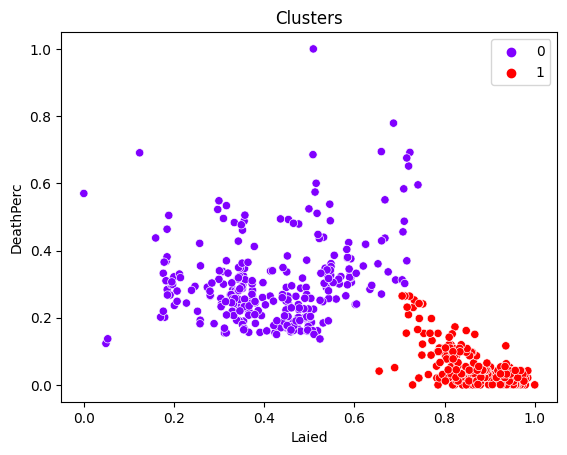
\includegraphics[width=70mm]
    {../Results/Two_clusters_division/CycleB/Hierarchical_scatter.png}}
         {Hierarchical cluster scatter plot}
    \\
    \hline
    \subf{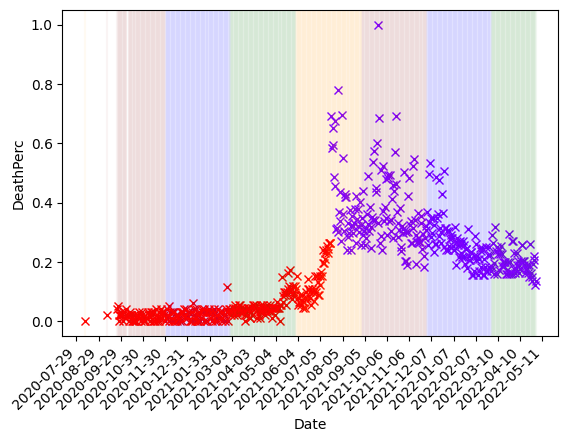
\includegraphics[width=70mm]
    {../Results/Two_clusters_division/CycleB/Hierarchical_plot_death.png}}
         {Percentage of death}
    &
    \subf{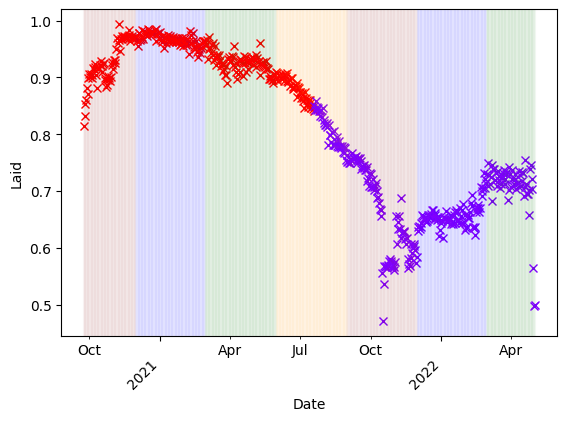
\includegraphics[width=70mm]
    {../Results/Two_clusters_division/CycleB/Hierarchical_plot_laied.png}}
         {Percentage of laid eggs}
    \\
    \hline
\end{tabular}
\end{center}

\subsection{Cycle C}
\begin{center}
    \begin{tabular}{| c | c | c | c | c | c | c |} 
        \hline
        Arrival date & \#Chickens & Frist Laid & End of cycle & Organic & \#Eggs\\ [0.5ex] 
        \hline
        20/06/2022 & 42.098 & 08/08/2022 & In progress & Yes & In progress\\ 
        \hline
    \end{tabular}
\end{center}

Significant features:
\begin{itemize}
    \item Average Percentage of Laid Eggs each day: 55,85\%
    \item Average Percentage of Death each day: 0,043\%
    \item Average Temperature during the cycle: 18,61 °C
    \item Average Humidity during the cycle: 70,05\%
\end{itemize}

Cluster:
\begin{center}
\begin{tabular}{|c|c|}
    \hline
    \subf{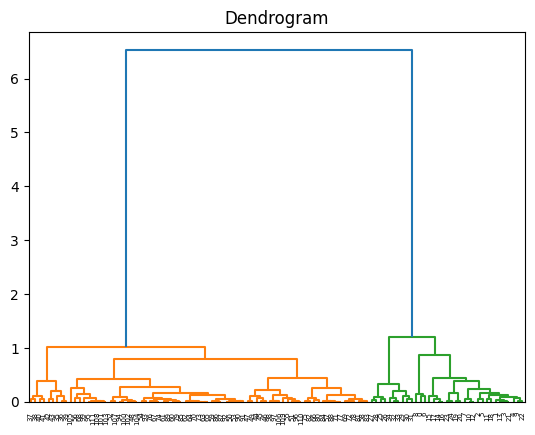
\includegraphics[width=70mm]
    {../Results/Two_clusters_division/CycleC/Hierarchical_dendogram.png}}
         {Dendogram}
    &
    \subf{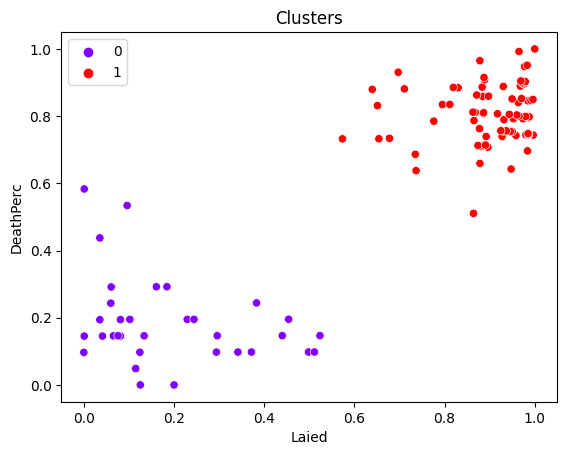
\includegraphics[width=70mm]
    {../Results/Two_clusters_division/CycleC/Hierarchical_scatter.png}}
         {Hierarchical cluster scatter plot}
    \\
    \hline
    \subf{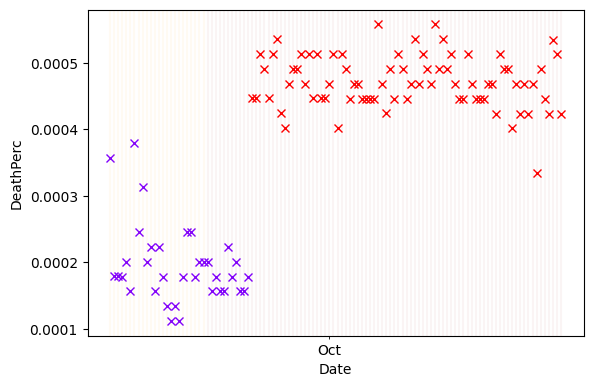
\includegraphics[width=70mm]
    {../Results/Two_clusters_division/CycleC/Hierarchical_plot_death.png}}
         {Percentage of death}
    &
    \subf{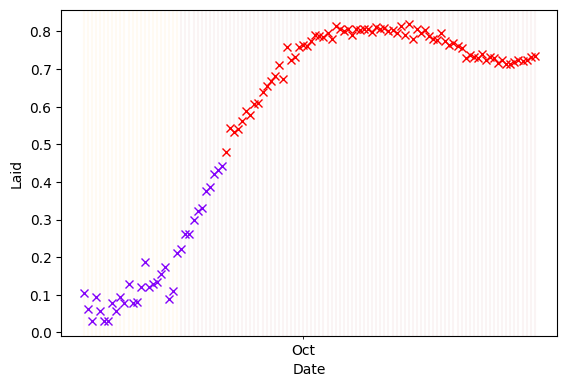
\includegraphics[width=70mm]
    {../Results/Two_clusters_division/CycleC/Hierarchical_plot_laied.png}}
         {Percentage of laid eggs}
    \\
    \hline
\end{tabular}
\end{center}

\subsection{Cycle X1}
\begin{center}
    \begin{tabular}{| c | c | c | c | c | c | c |} 
        \hline
        Arrival date & \#Chickens & Frist Laid & End of cycle & Organic & \#Eggs\\ [0.5ex] 
        \hline
        20/01/2014 & 33.743 & 18/03/2014 & 08/07/2015 & No & 12.375.840\\ 
        \hline
    \end{tabular}
\end{center}

Significant features:
\begin{itemize}
    \item Average Percentage of Laid Eggs each day: 80,69\%
    \item Average Percentage of Death each day: 0,032\%
    \item Average Temperature during the cycle: 15,34 °C
    \item Average Humidity during the cycle: 72,83\%
\end{itemize}

Cluster:
\begin{center}
\begin{tabular}{|c|c|}
    \hline
    \subf{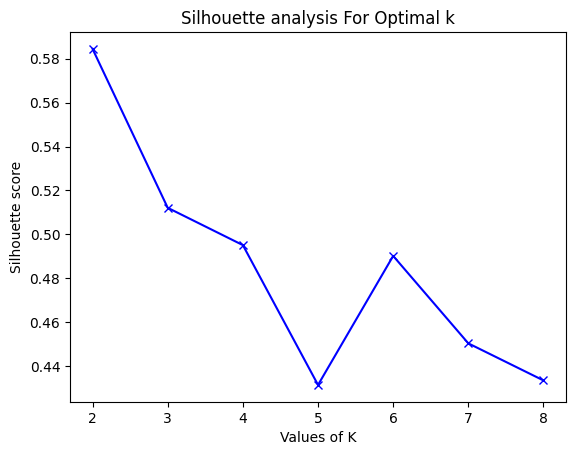
\includegraphics[width=70mm]
    {../Results/Two_clusters_division/CycleX1/KMeans_silhouette.png}}
         {Silhouette}
    &
    \subf{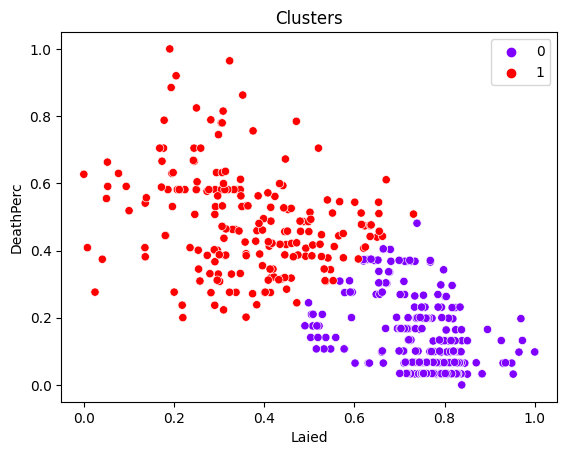
\includegraphics[width=70mm]
    {../Results/Two_clusters_division/CycleX1/KMeans_scatter.png}}
         {K-Means cluster scatter plot}
    \\
    \hline
    \subf{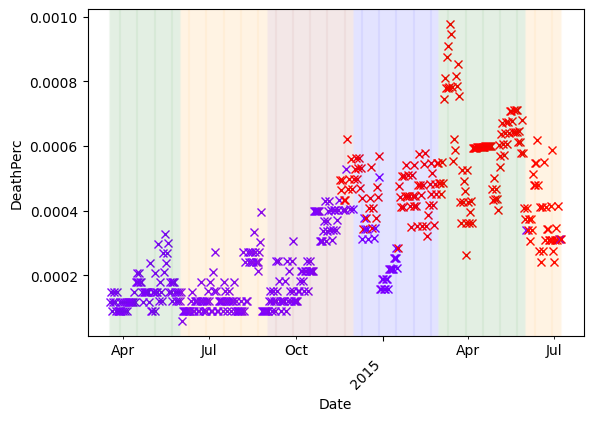
\includegraphics[width=70mm]
    {../Results/Two_clusters_division/CycleX1/KMeans_plot_death.png}}
         {Percentage of death}
    &
    \subf{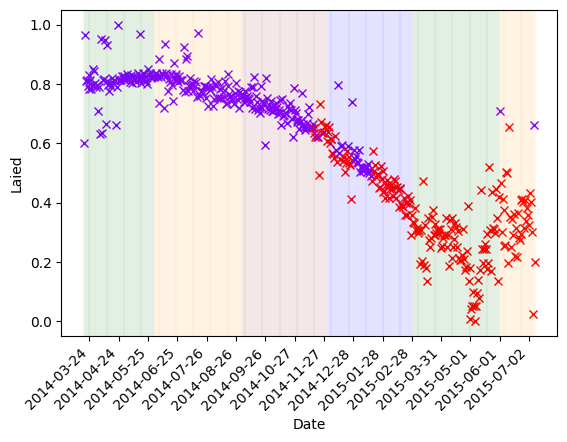
\includegraphics[width=70mm]
    {../Results/Two_clusters_division/CycleX1/KMeans_plot_laied.png}}
         {Percentage of laid eggs}
    \\
    \hline
\end{tabular}
\end{center}

\subsection{Cycle X2}
\begin{center}
    \begin{tabular}{| c | c | c | c | c | c | c |} 
        \hline
        Arrival date & \#Chickens & Frist Laid & End of cycle & Organic & \#Eggs\\ [0.5ex] 
        \hline
        26/05/2014 & 23.898 & 15/07/2014 & 21/06/2015 & No & 7.558.799\\ 
        \hline
    \end{tabular}
\end{center}

Significant features:
\begin{itemize}
    \item Average Percentage of Laid Eggs each day: 95,36\%
    \item Average Percentage of Death each day: 0,021\%
    \item Average Temperature during the cycle: 13,76 °C
    \item Average Humidity during the cycle: 76,04\%
\end{itemize}

Cluster:
\begin{center}
\begin{tabular}{|c|c|}
    \hline
    \subf{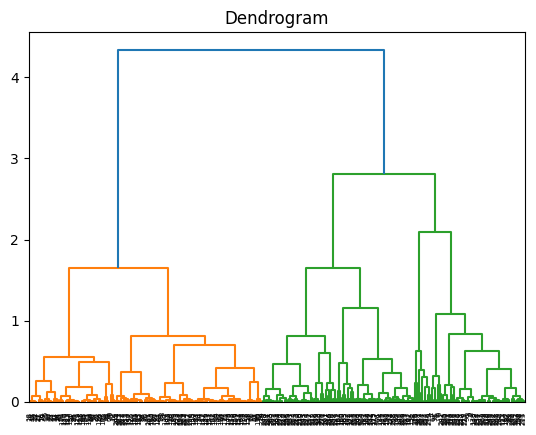
\includegraphics[width=70mm]
    {../Results/Two_clusters_division/CycleX2/Hierarchical_dendogram.png}}
         {Dendogram}
    &
    \subf{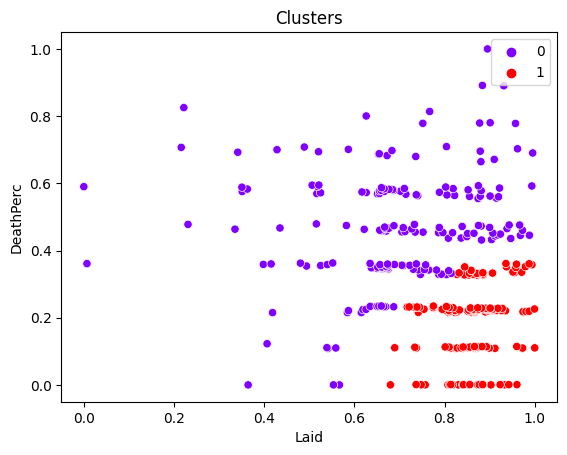
\includegraphics[width=70mm]
    {../Results/Two_clusters_division/CycleX2/Hierarchical_scatter.png}}
         {Hierarchical cluster scatter plot}
    \\
    \hline
    \subf{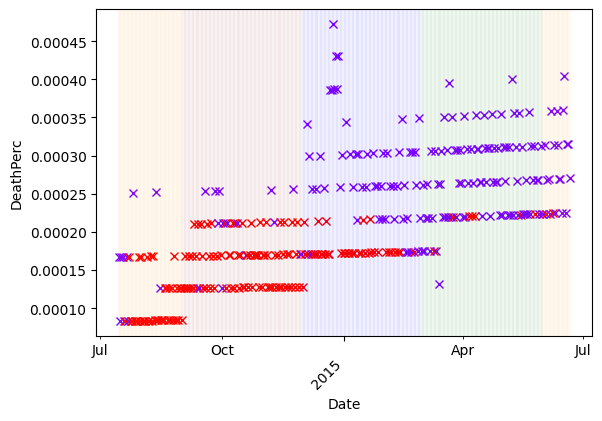
\includegraphics[width=70mm]
    {../Results/Two_clusters_division/CycleX2/Hierarchical_plot_death.png}}
         {Percentage of death}
    &
    \subf{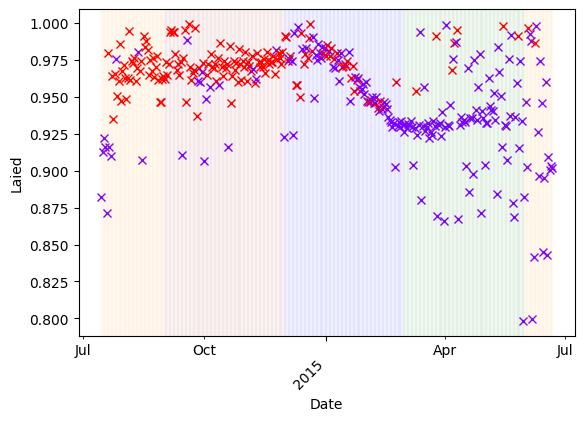
\includegraphics[width=70mm]
    {../Results/Two_clusters_division/CycleX2/Hierarchical_plot_laied.png}}
         {Percentage of laid eggs}
    \\
    \hline
\end{tabular}
\end{center}

\subsection{Cycle Y}
\begin{center}
    \begin{tabular}{| c | c | c | c | c | c | c |} 
        \hline
        Arrival date & \#Chickens & Frist Laid & End of cycle & Organic & \#Eggs\\ [0.5ex] 
        \hline
        11/08/2015 & 57.346 & 05/10/2015 & 27/09/2016 & No & 16.759.240\\ 
        \hline
    \end{tabular}
\end{center}

Significant features:
\begin{itemize}
    \item Average Percentage of Laid Eggs each day: 83.70\%
    \item Average Percentage of Death each day: 0,022\%
    \item Average Temperature during the cycle: 14,20 °C
    \item Average Humidity during the cycle: 74,54\%
\end{itemize}

Cluster:
\begin{center}
\begin{tabular}{|c|c|}
    \hline
    \subf{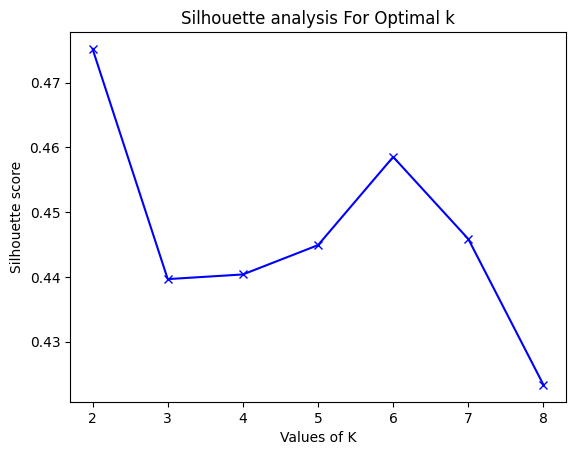
\includegraphics[width=70mm]
    {../Results/Two_clusters_division/CycleY/KMeans_silhouette.png}}
         {Silhouette}
    &
    \subf{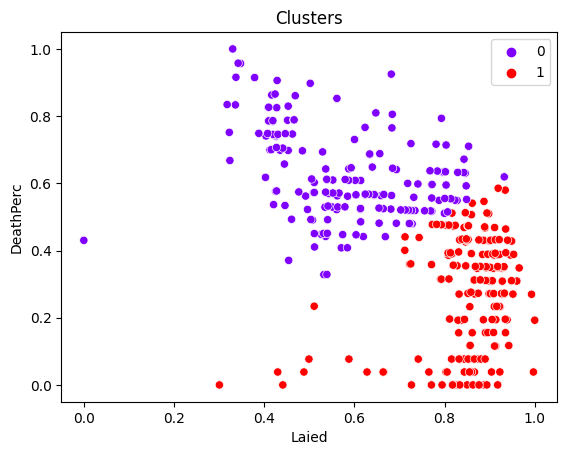
\includegraphics[width=70mm]
    {../Results/Two_clusters_division/CycleY/KMeans_scatter.png}}
         {K-means cluster scatter plot}
    \\
    \hline
    \subf{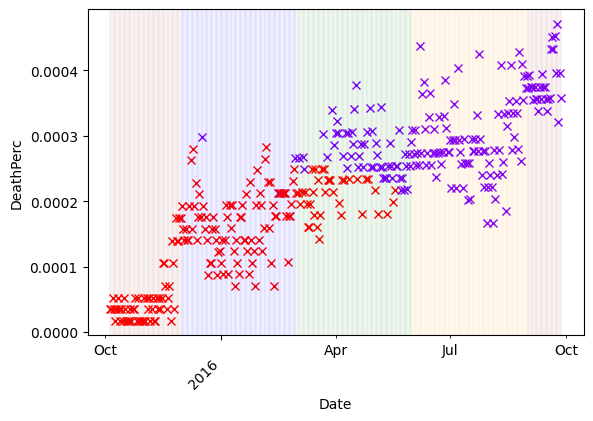
\includegraphics[width=70mm]
    {../Results/Two_clusters_division/CycleY/KMeans_plot_death.png}}
         {Percentage of death}
    &
    \subf{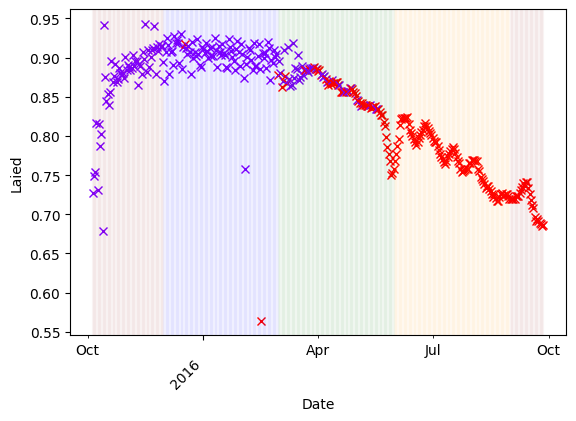
\includegraphics[width=70mm]
    {../Results/Two_clusters_division/CycleY/KMeans_plot_laied.png}}
         {Percentage of laid eggs}
    \\
    \hline
\end{tabular}
\end{center}

\subsection{Cycle Z}
\begin{center}
    \begin{tabular}{| c | c | c | c | c | c | c |} 
        \hline
        Arrival date & \#Chickens & Frist Laid & End of cycle & Organic & \#Eggs\\ [0.5ex] 
        \hline
        17/11/2016 & 42.130 & 08/01/2017 & 27/05/2018 & Yes & 17.721.240\\ 
        \hline
    \end{tabular}
\end{center}

Significant features:
\begin{itemize}
    \item Average Percentage of Laid Eggs each day: 87,78\%
    \item Average Percentage of Death each day: 0,021\%
    \item Average Temperature during the cycle: 13,07 °C
    \item Average Humidity during the cycle: 74,27\%
\end{itemize}

Cluster:
\begin{center}
\begin{tabular}{|c|c|}
    \hline
    \subf{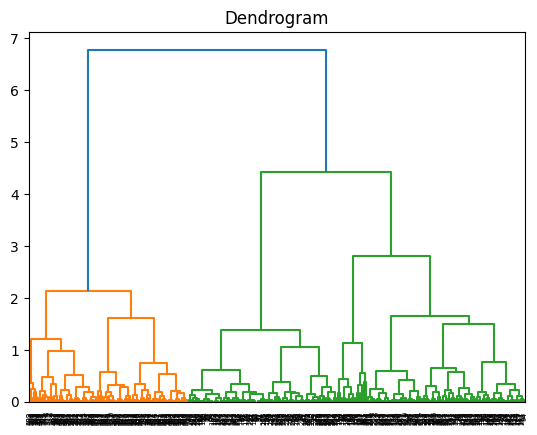
\includegraphics[width=70mm]
    {../Results/Two_clusters_division/CycleZ/Hierarchical_dendogram.png}}
         {Dendogram}
    &
    \subf{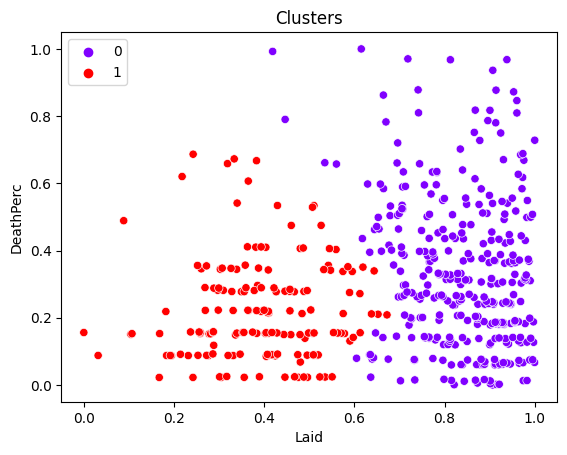
\includegraphics[width=70mm]
    {../Results/Two_clusters_division/CycleZ/Hierarchical_scatter.png}}
         {Hierarchical cluster scatter plot}
    \\
    \hline
    \subf{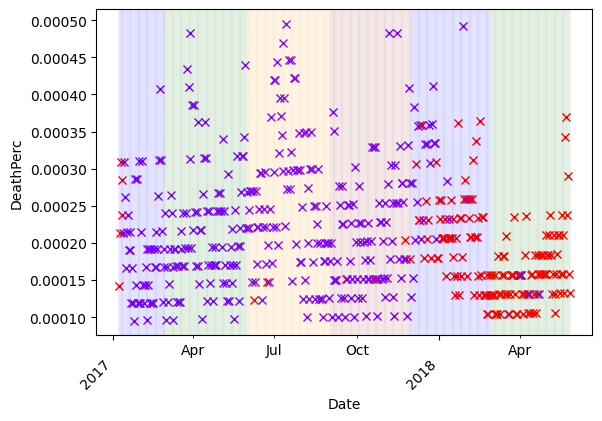
\includegraphics[width=70mm]
    {../Results/Two_clusters_division/CycleZ/Hierarchical_plot_death.png}}
         {Percentage of death}
    &
    \subf{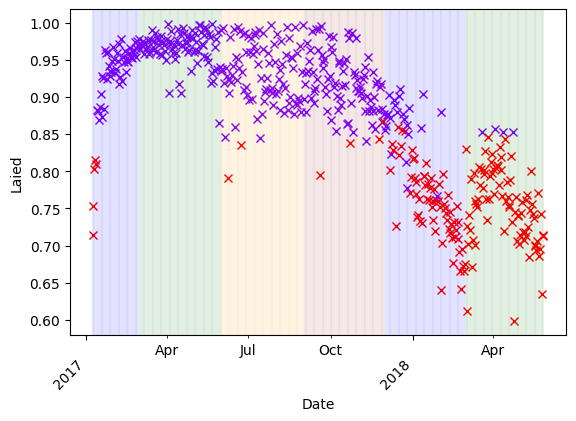
\includegraphics[width=70mm]
    {../Results/Two_clusters_division/CycleZ/Hierarchical_plot_laied.png}}
         {Percentage of laid eggs}
    \\
    \hline
\end{tabular}
\end{center}

\section{Common features}
In this section, we will discuss what we discovered by comparing all the cycles together.
After seeing that each cycle can be clustered in two parts, those clusters also divide the cycle into two distinct sections in a plot based on date. We tried to apply the same idea in a dataset composed of all the cycles together.

\begin{center}
    \begin{tabular}{|c|c|}
        \hline
        \subf{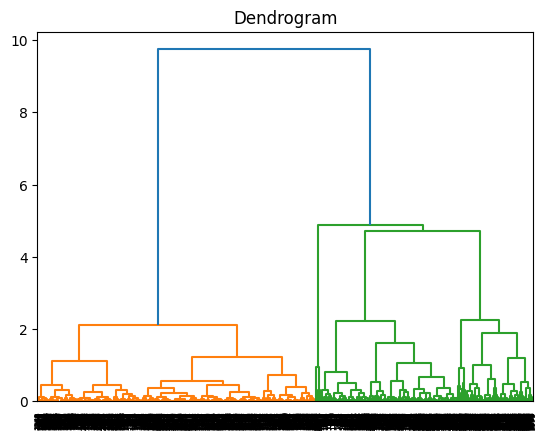
\includegraphics[width=70mm]
        {../Results/Every_cycle/Hierarchical_dendogram.png}}
             {Dendogram}
        &
        \subf{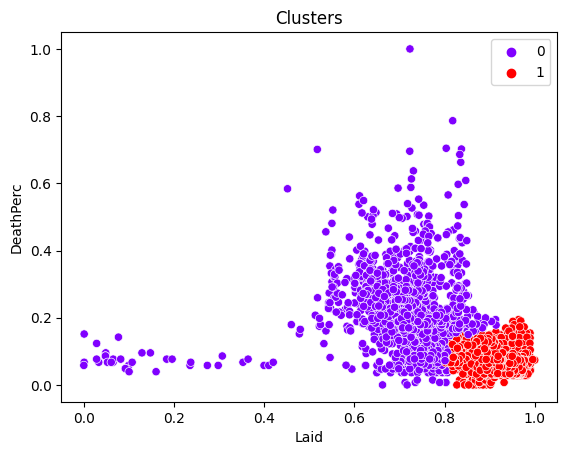
\includegraphics[width=70mm]
        {../Results/Every_cycle/Hierarchical_scatter_death.png}}
             {Hierarchical cluster scatter plot}
    \end{tabular}
    \begin{tabular}{|c|}
        \hline
        \subf{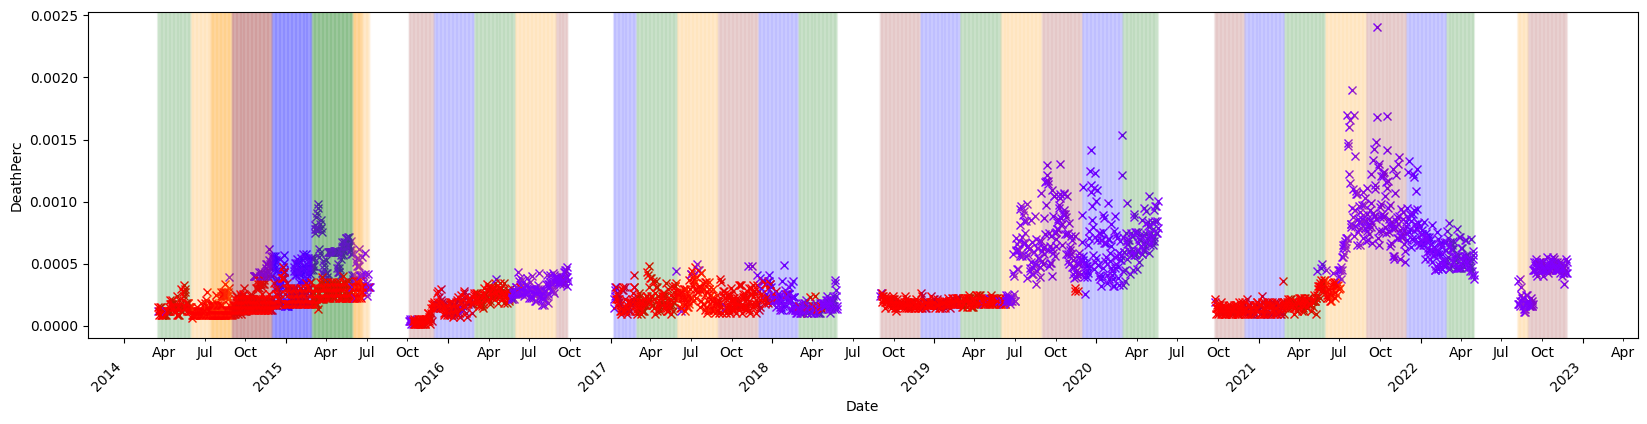
\includegraphics[width=144mm]
    {../Results/Every_cycle/Hierarchical_plot_death.png}}
         {Percentage of death}\\
    \hline
    \subf{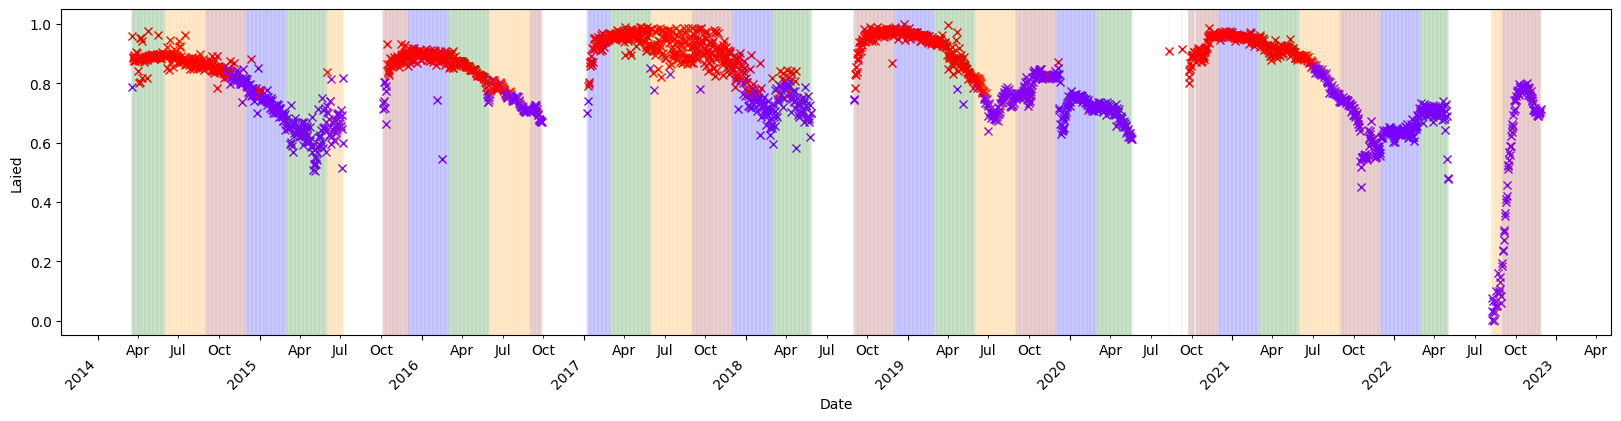
\includegraphics[width=144 mm]
    {../Results/Every_cycle/Hierarchical_plot_laied.png}}
         {Percentage of laid eggs}
    \\
    \hline
    \end{tabular}
    
\end{center}

Looking at the clusters we find that indeed the division of each cycle is respected. We find also that the only one that didn't respect this division is cycle C, which could be expected since it just started, but the interesting thing is that the whole cycle C is clustered as cluster 1 which is the one that identifies the end of every other cycle so we can see how bad is performing this new cycle both in death and laid rate.
This can show how the ban on beak-cutting affected the welfare of the chickens, with the beak the violence between animals increased a lot and not only increase the death rate but increased a lot the stress of the chickens reducing their productivity.

To better compare the different cycles we made a spider plot with 4 features:
\begin{itemize}
    \item Average Percentage of Laid Eggs each day
    \item Average Percentage of Death each day
    \item Average Temperature during the cycle
    \item Average Humidity during the cycle
\end{itemize}
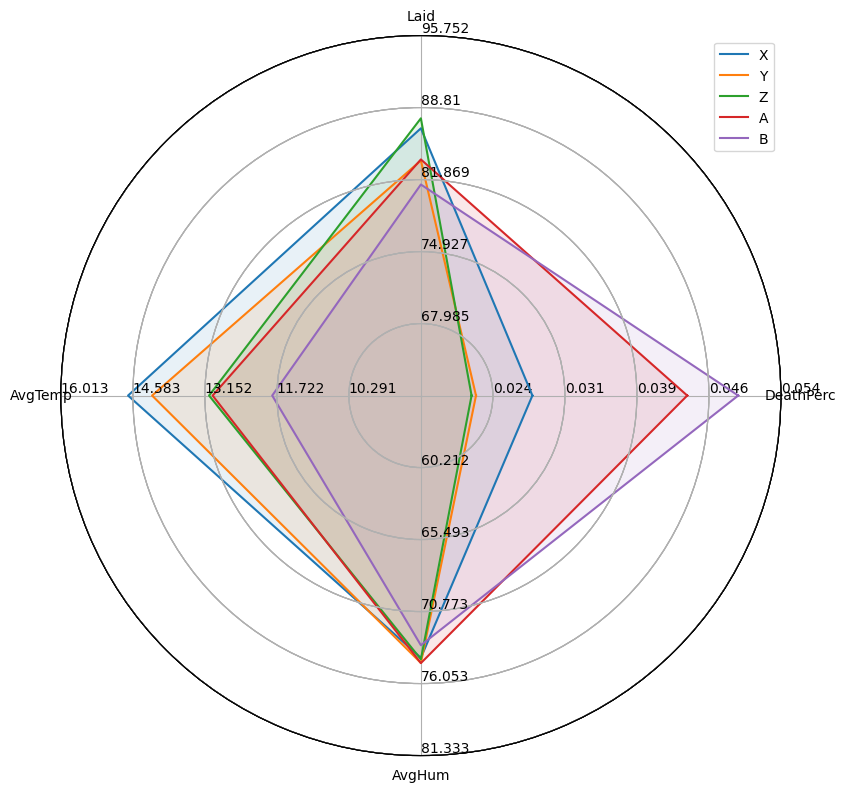
\includegraphics[width=\linewidth]{../Results/Every_cycle/Spider_Plot.png}
\section{Organic vs non-organic cycles}

\section{Death-season correlation}

\section{Economic results}

\end{document}